% !TeX root = ../presentation.tex

\section{Introduction}
\begin{frame}{What is interpolation?}
	\begin{columns}[T] % align columns
		\begin{column}{.48\textwidth}
			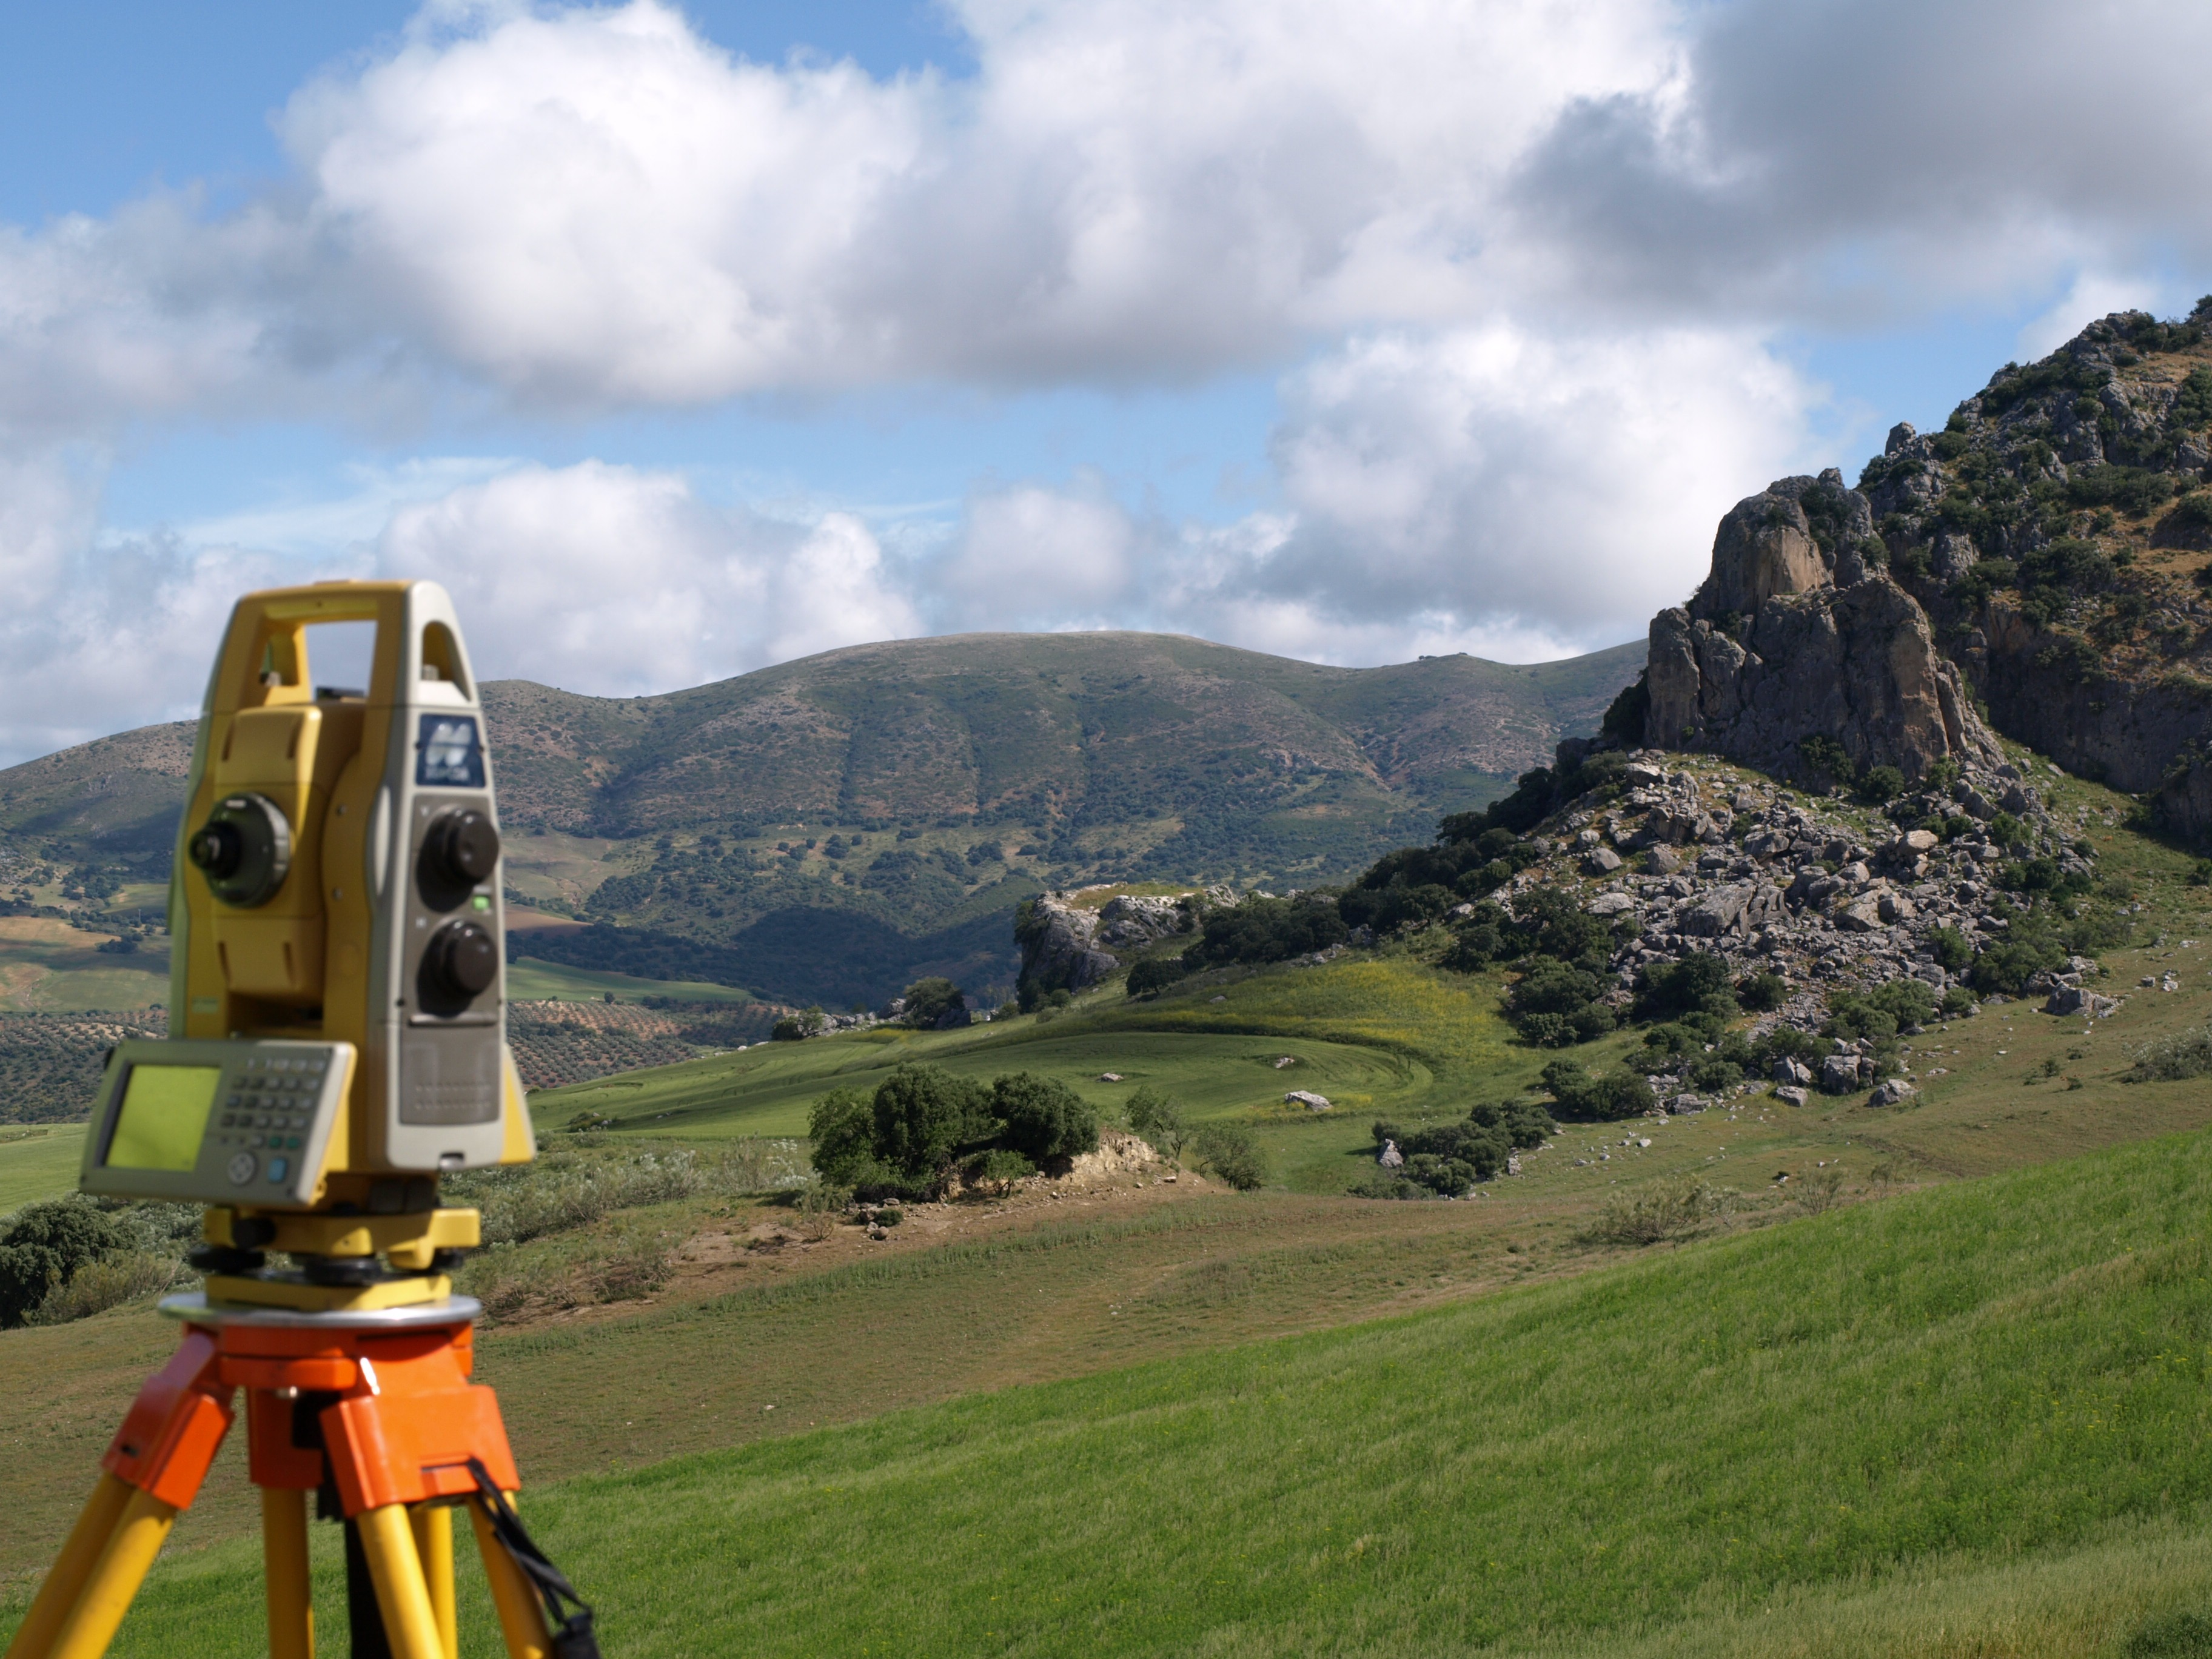
\includegraphics[width=\linewidth]{images/background}
		\end{column}%
		\hfill%
		\begin{column}{.56\textwidth}
			\begin{itemize}
				\item TODO
				\item TODO 2
			\end{itemize}
		\end{column}%
	\end{columns}
	\note{say "hello" now}
\end{frame}
\begin{frame}{This is interpolation!}
\begin{columns}[T] % align columns
	\begin{column}{.56\textwidth}
		\begin{itemize}
			\item TODO
		\end{itemize}
	\end{column}%
	\hfill%
	\begin{column}{.48\textwidth}
		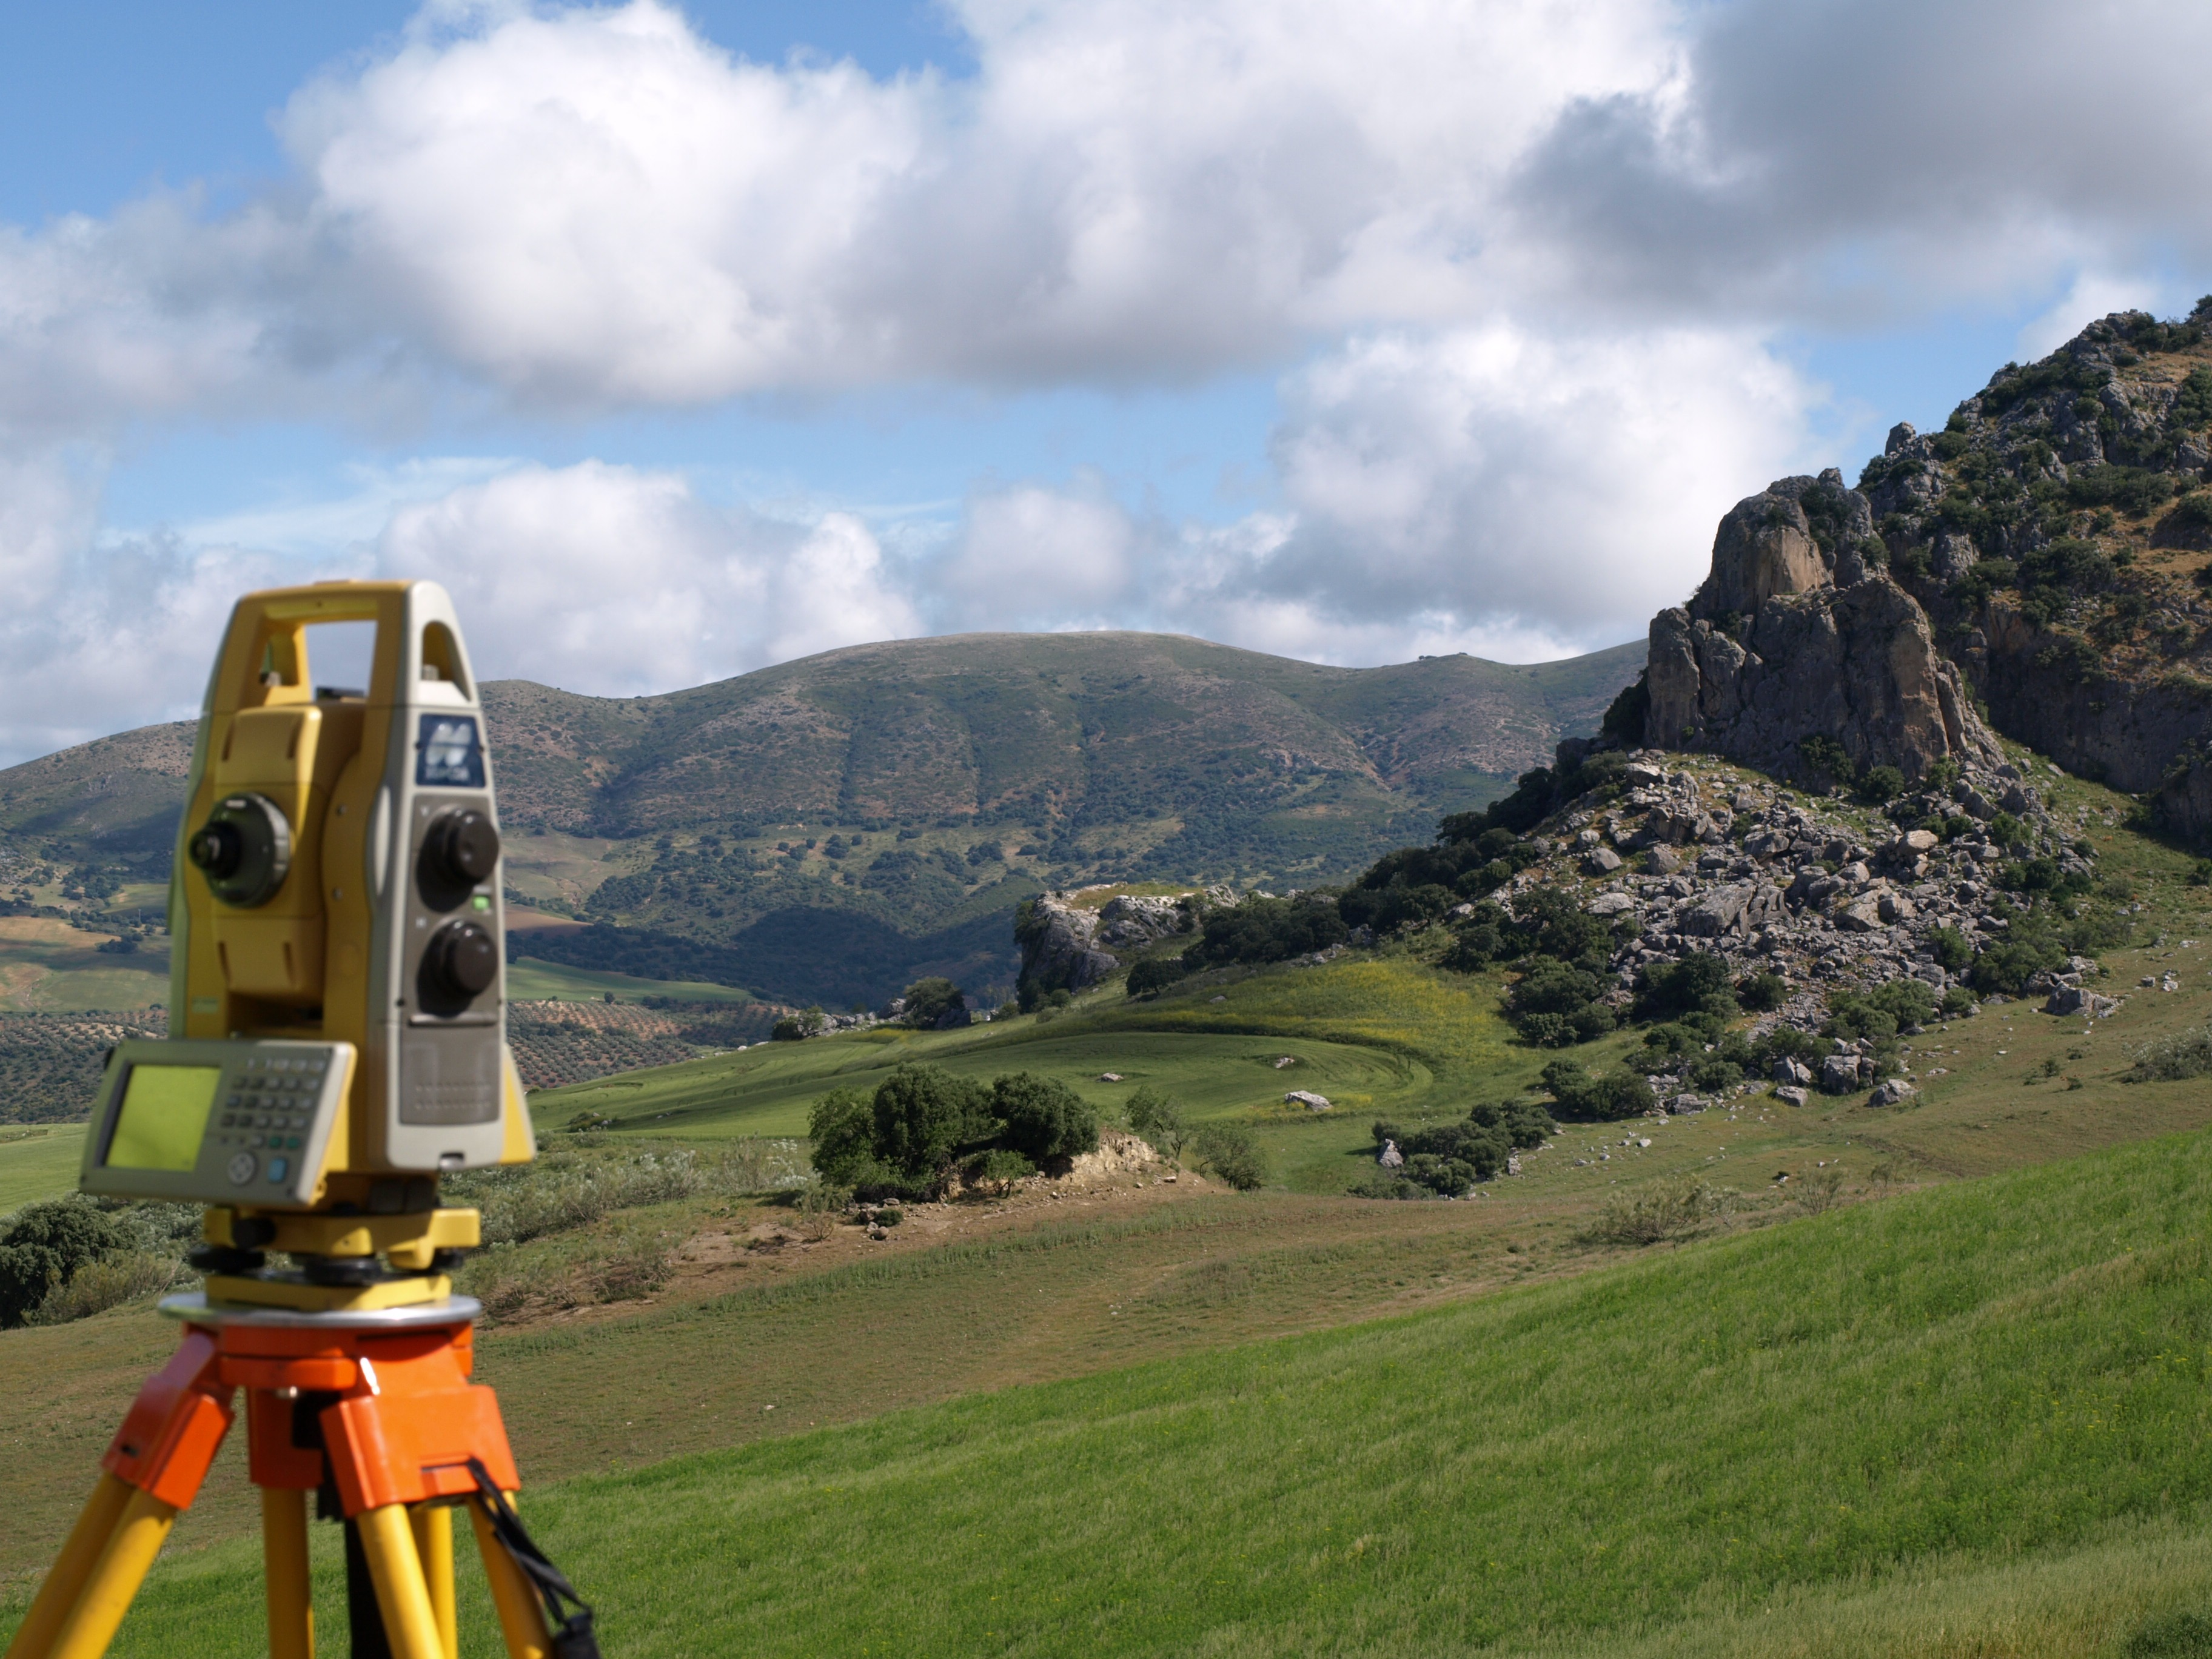
\includegraphics[width=\linewidth]{images/background}
	\end{column}%
\end{columns}
\note{say "hello" now}
\end{frame}